\section*{Bestemmelse af forskrift for en eksponentiel funktion ud fra datasæt}

For at bestemme forskriften for den eksponentielle funktion, $y = b\cdot a^x$ skal vi bruge følgende formler til at bestemme a og b

\begin{frm-thm}{Bestemmelse af forskrift for den eksponentielle funktion}

Givet 2 datapunkter $(x_1, y_1)$ og $(x_2, y_2)$ kan a og b værdien for den eksponentielle funktions forskrifte bestemmes ved

\begin{align*}
a = \sqrt[x_2 - x_1]{\frac{y_2}{y_1}}
\end{align*}

\[b = \frac{y_1}{a^{x_1}}\]

\end{frm-thm}


Vi vil nu se på et eksempel.


\textbf{Eksempel:}

Vi er givet datasættet 

\begin{tabular}{c|c|c|c|c|c|c}
x & 0 & 1 & 2 & 3 & 4 & 5 \\\hline
y & 10 & 20 & 40 & 80 & 160 & 320
\end{tabular}

Vi bestemmer først a værdien, og udvælger de første 2 kolonner i datasættet som vores datapunkter, $(x_1, y_1) = (0, 10)$, $(x_2, y_2) = (1, 20)$.

Vi beregner nu a ud fra formlen 

\begin{align*}
a = \sqrt[x_2 - x_1]{\frac{y_2}{y_1}} = \sqrt[1 - 0]{\frac{20}{10}} = \sqrt[1]{2} = 2
\end{align*}

Så a værdien for den eksponentielle funktion er dermed 2.

Vi bestemmer nu b ved brug af formlen og får

\begin{align*}
b = \frac{y_1}{a^{x_1}} = \frac{10}{2^0} = \frac{10}{1} = 10
\end{align*}

Så b værdien for den eksponentielle funktion er dermed 10, og vi får forskriften for den eksponentielle funktion til følgende

\begin{align*}
y = 10\cdot 2^x
\end{align*}

\newpage 

Vi vil nu vise hvordan man bestemmer forskriften for den eksponentielle funktion ud fra datasættet i GeoGebra

Først vælger vi regneark og indtaster x værdierne i A kolonnen og y værdierne i B kolonnen, hvorefter vi markerer de 2 kolonner som kan ses på nedenstående figur

\begin{figure*}[ht]
    \centering
    \begin{subfigure}[t]{0.5\textwidth}
        \centering
        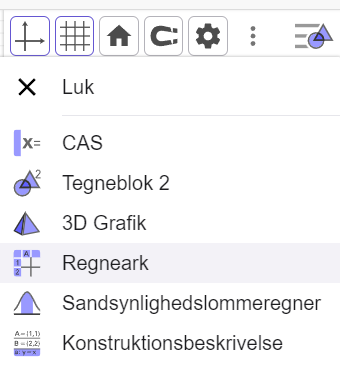
\includegraphics[width=0.35\textwidth]{img_1}
        \caption{Regneark vælges}
    \end{subfigure}%
    ~ 
    \begin{subfigure}[t]{0.5\textwidth}
        \centering
        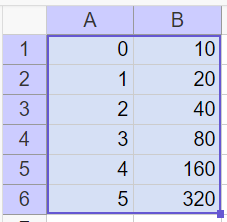
\includegraphics[width=0.35\textwidth]{img_2}
        \caption{Regneark med A og B kolonnerne udfyldt med x og y værdierne}
    \end{subfigure}
    \caption{Bestemmelse af forskrift for eksponentiel funktion ud fra datasæt}
\end{figure*}

Herefter vælger vi regressionsanalyse og får følgende plot frem

\begin{figure*}[ht]
    \centering
    \begin{subfigure}[t]{0.5\textwidth}
        \centering
        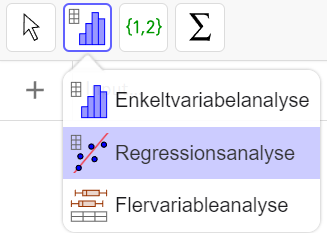
\includegraphics[width=0.5\textwidth]{img_3}
        \caption{Regressionsanalyse vælges}
    \end{subfigure}%
    ~ 
    \begin{subfigure}[t]{0.5\textwidth}
        \centering
        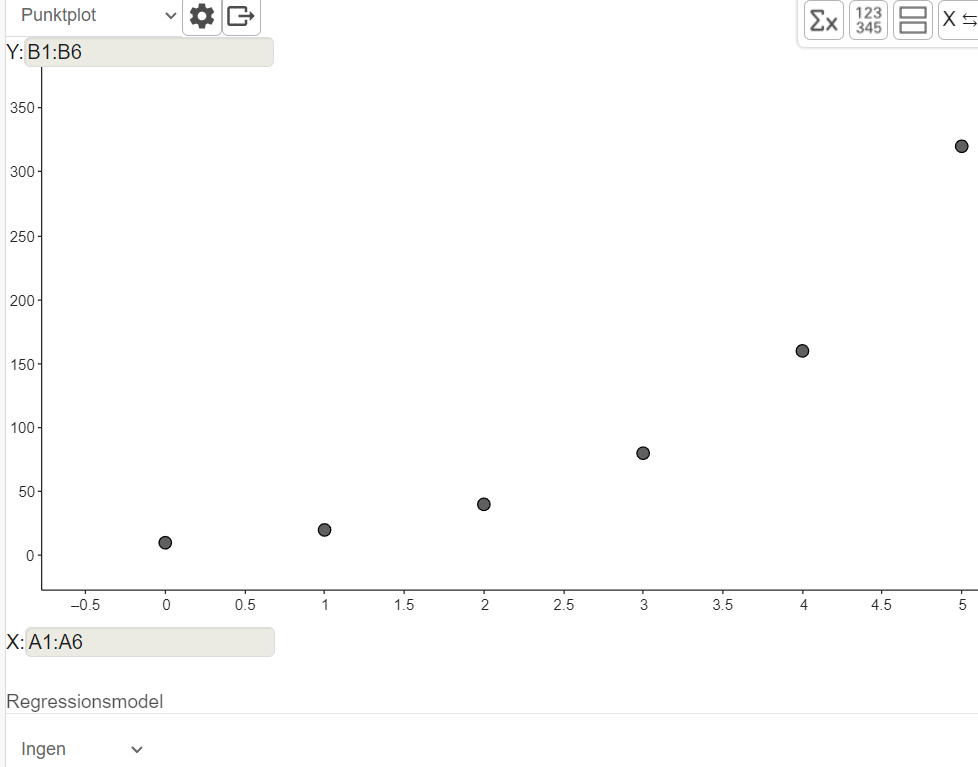
\includegraphics[width=0.5\textwidth]{img_4}
        \caption{Plot over datasættet}
    \end{subfigure}
    \caption{Bestemmelse af forskrift for eksponentiel funktion ud fra datasæt}
\end{figure*}


Derefter vælger vi regressionsmodellen vækst og får plottet linjen, som på plottet har forskriften $y = 10\cdot 2^x$

\begin{figure*}[ht]
    \centering
    \begin{subfigure}[t]{0.5\textwidth}
        \centering
        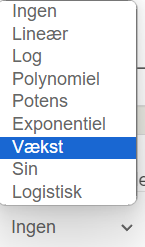
\includegraphics[width=0.3\textwidth]{img_5}
        \caption{Regressionsmodellen vækst vælges}
    \end{subfigure}%
    ~ 
    \begin{subfigure}[t]{0.5\textwidth}
        \centering
        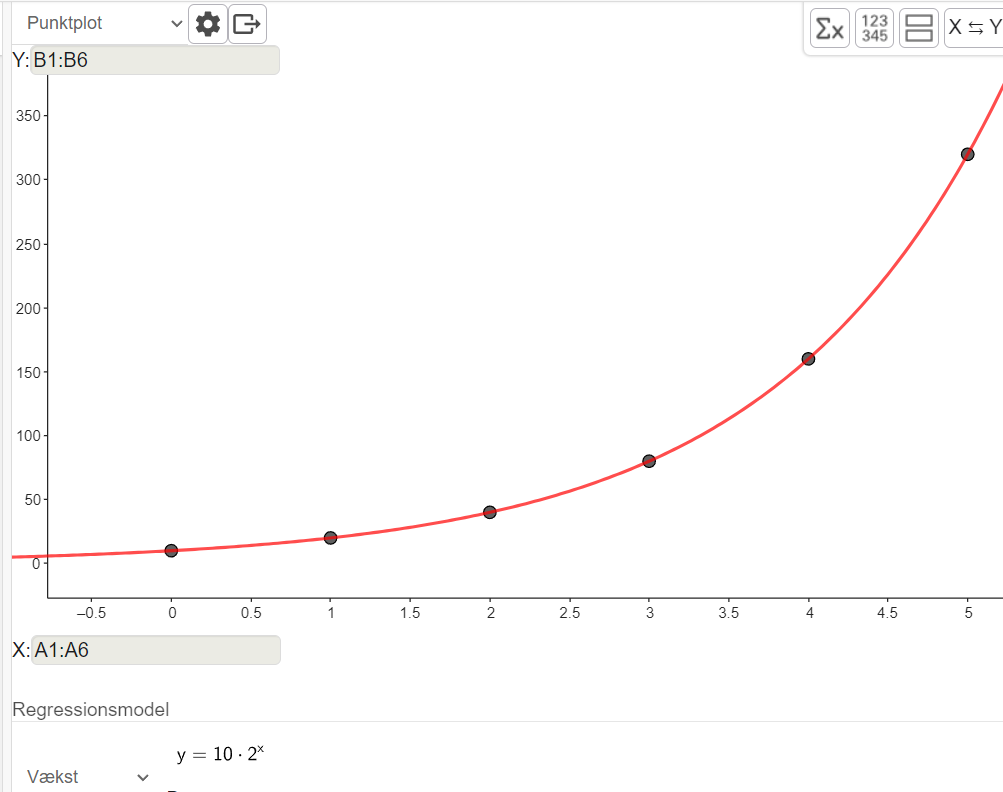
\includegraphics[width=0.6\textwidth]{img_6}
        \caption{Det endelige plot med forskriften for den eksponentielle funktion}
    \end{subfigure}
    \caption{Bestemmelse af forskrift for eksponentiel funktion ud fra datasæt}
\end{figure*}


\newpage

\subsection*{Opgaver}



\textbf{Opgave 1:}

Bestem forskriften for den eksponentielle funktion der passer på følgende datasæt
\begin{tabular}{c|c|c|c|c|c|c}
x & 0 & 2 & 4 & 6 & 8 & 10 \\\hline
y & 4 & 8 & 16 & 32 & 64 & 128
\end{tabular}

\textbf{Opgave 2:}

Bestem forskriften for den eksponentielle funktion der passer på følgende datasæt
\begin{tabular}{c|c|c|c|c|c|c}
x & 0 & 20 & 40 & 60 & 80 & 100 \\\hline
y & 60 & 120 & 240 & 480 & 960 & 1920
\end{tabular}

\textbf{Opgave 3:}

Bestem forskriften for den eksponentielle funktion der passer på følgende datasæt
\begin{tabular}{c|c|c|c|c|c|c}
x & 0 & 5 & 10 & 15 & 20 & 25 \\\hline
y & 80 & 160 & 320 & 640 & 1280 & 2560
\end{tabular}

\textbf{Opgave 4:}

Bestem forskriften for den eksponentielle funktion der passer på følgende datasæt
\begin{tabular}{c|c|c|c|c|c|c}
x & 0 & 3 & 6 & 9 & 12 & 15 \\\hline
y & 128 & 64 & 32 & 16 & 8 & 4
\end{tabular}

\textbf{Opgave 5:}

Bestem forskriften for den eksponentielle funktion der passer på følgende datasæt
\begin{tabular}{c|c|c|c|c|c|c}
x & 0 & 4 & 8 & 12 & 16 & 20 \\\hline
y & 1000 & 500 & 250 & 125 & 62.5 & 31.25
\end{tabular}




\newpage


\subsection*{Facit}


\textbf{Opgave 1:}

\begin{figure}[ht]
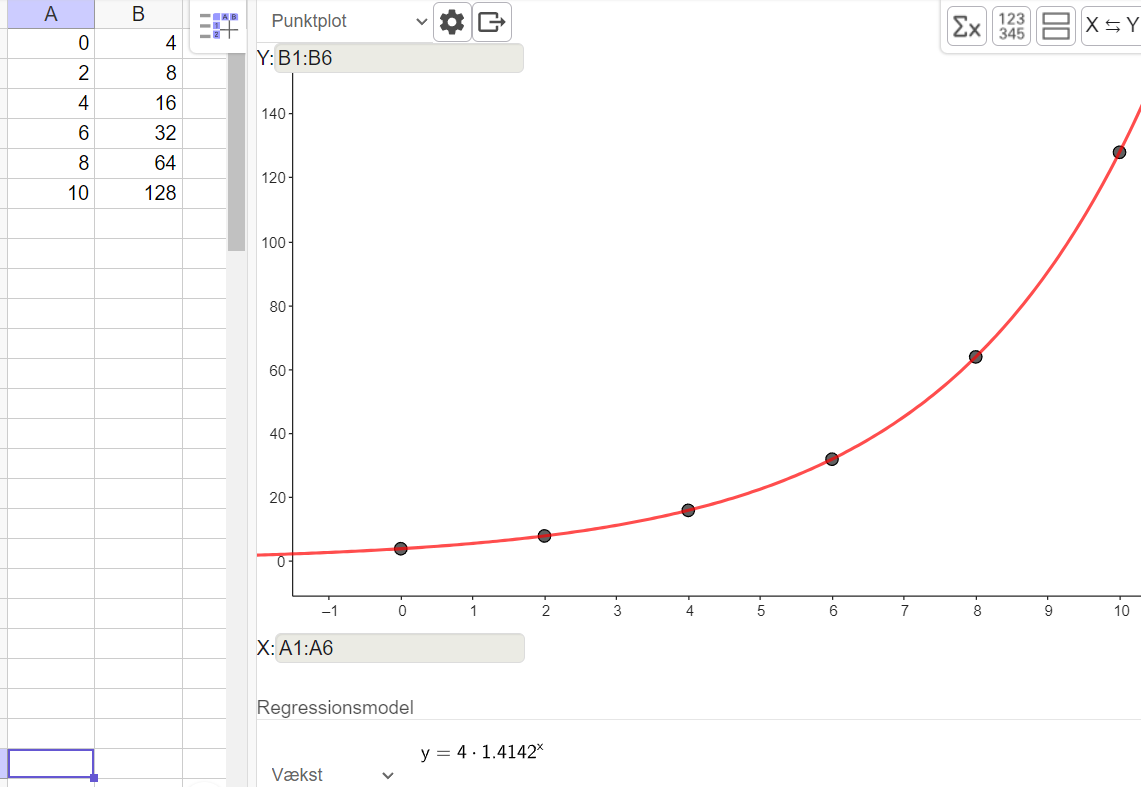
\includegraphics[width=0.62\textwidth, height=0.27\textwidth]{ans_1}
\caption{Den eksponentielle funktion med forskriften $y = 4\cdot 1.4142^x$}
\end{figure}

\textbf{Opgave 2:}

\begin{figure}[ht]
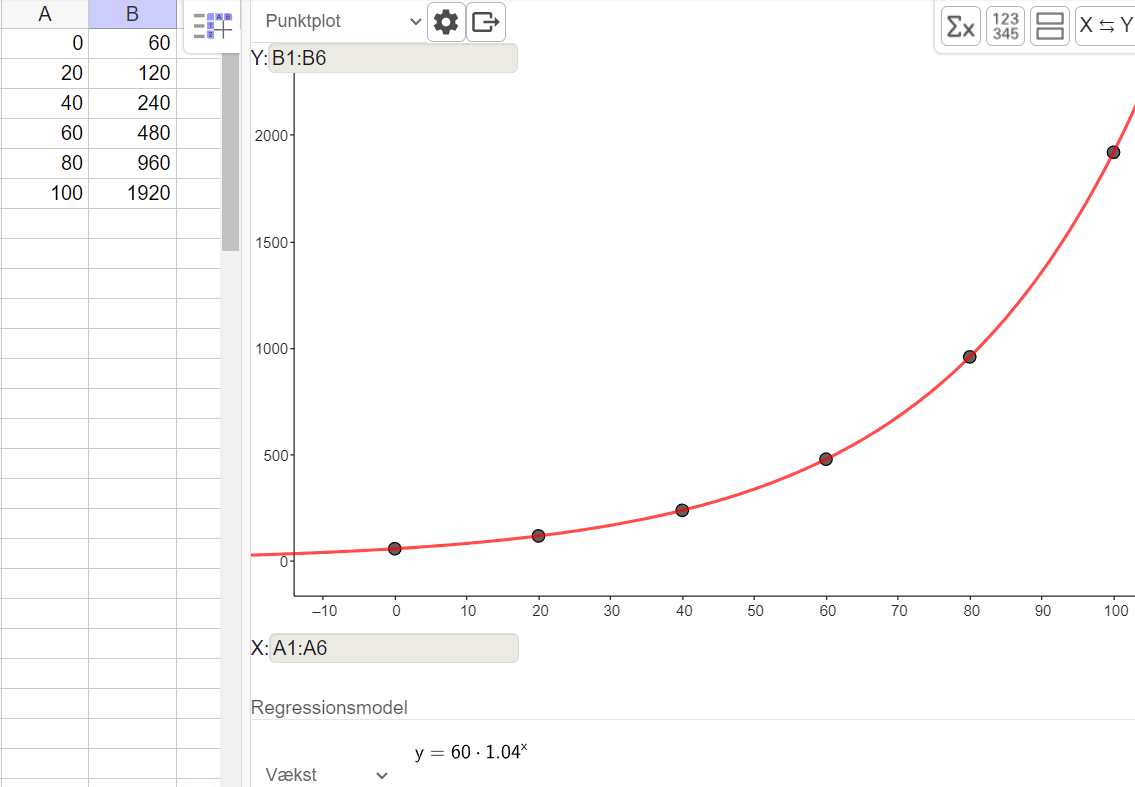
\includegraphics[width=0.62\textwidth, height=0.27\textwidth]{ans_2}
\caption{Den eksponentielle funktion med forskriften $y = 60\cdot 1.04^x$}
\end{figure}

\textbf{Opgave 3:}

\begin{figure}[ht]
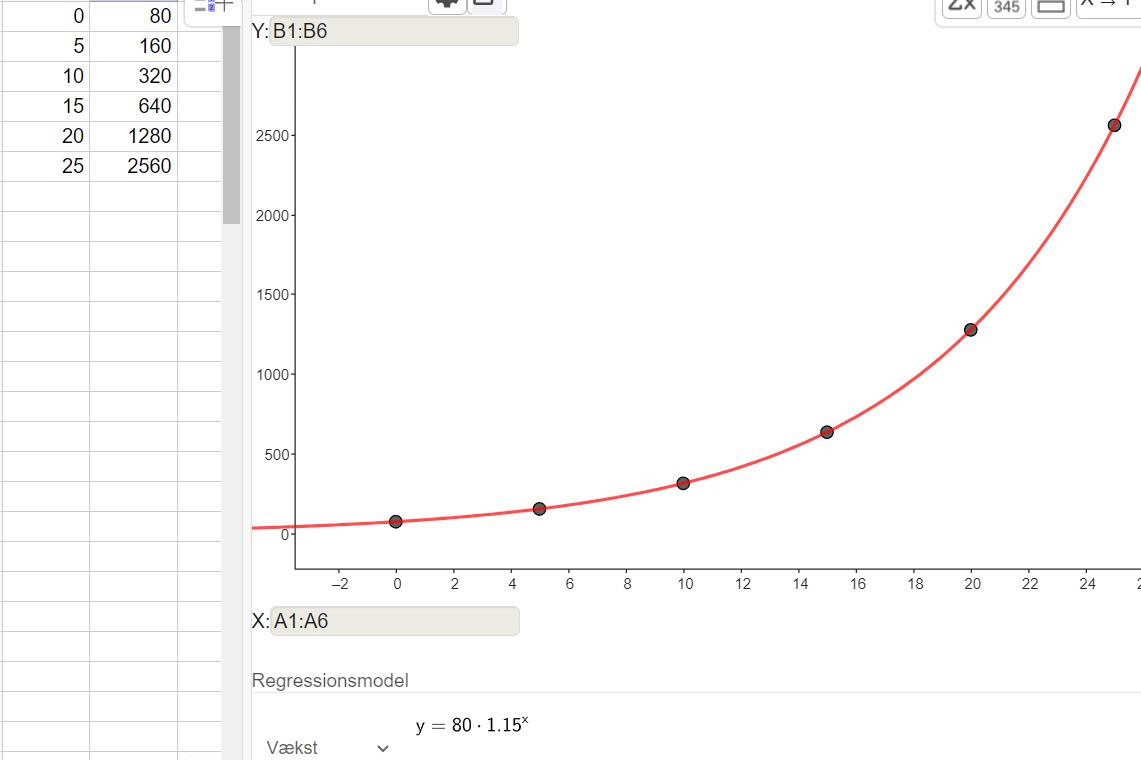
\includegraphics[width=0.62\textwidth, height=0.27\textwidth]{ans_3}
\caption{Den eksponentielle funktion med forskriften $y = 80 \cdot 1.15^x$}
\end{figure}

\newpage

\textbf{Opgave 4:}

\begin{figure}[ht]
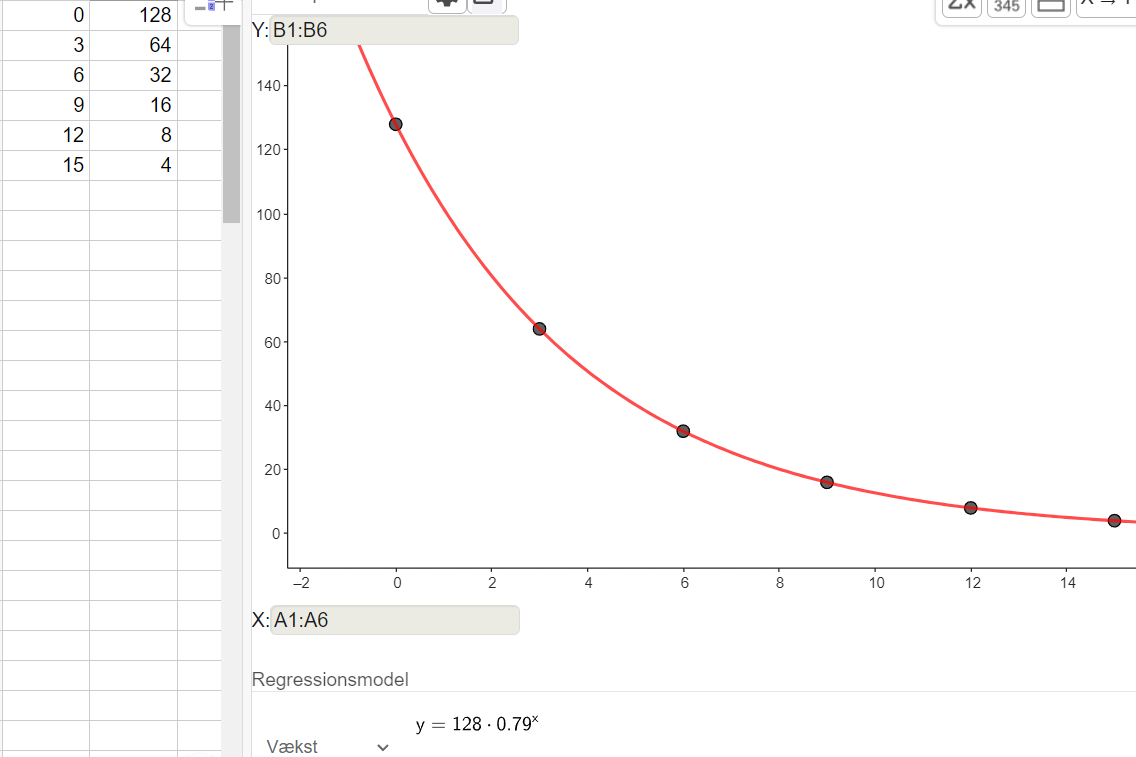
\includegraphics[width=0.62\textwidth, height=0.27\textwidth]{ans_4}
\caption{Den eksponentielle funktion med forskriften $y =128\cdot 0.79^x $}
\end{figure}

\textbf{Opgave 5:}

\begin{figure}[ht]
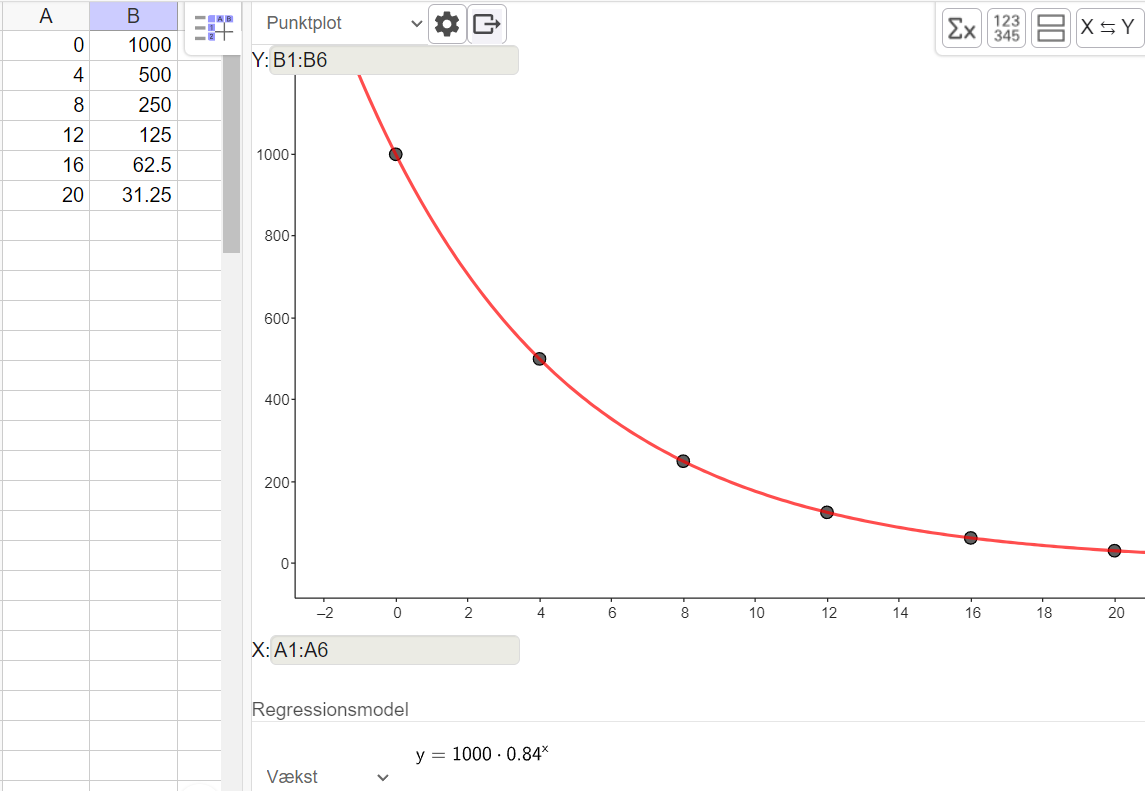
\includegraphics[width=0.62\textwidth, height=0.27\textwidth]{ans_5}
\caption{Den eksponentielle funktion med forskriften $y = 1000\cdot 0.84^x$}
\end{figure}